\documentclass[11pt]{report}
\usepackage{amsfonts, amsmath, amssymb}
\usepackage{tikz}
\usepackage[framemethod=tikz]{mdframed}
\usepackage{float}
\usepackage{hyperref}
\usepackage{url}
\usepackage{fancyhdr}
\usepackage[none]{hyphenat}
\usepackage{listings}
\usepackage{xcolor}
\usepackage{tabularx}
\usepackage[nottoc, notlot, notlof]{tocbibind}
\usepackage[comma]{natbib}
\usepackage{nicematrix}
\usepackage{tabularray}
\usepackage{todonotes}
\usepackage{minted}
\usepackage{fontawesome5}
\usepackage{currfile}
\usepackage{xstring}
\usepackage{alltt} 
\usepackage[all]{nowidow}
\usepackage{color,soul}
\usepackage[acronym]{glossaries}
\usepackage{comment}

% definitions
\def\papertitle{Syntatic and Semantic Considerations for Parallel Compilation}
% Alternate title: Lexical and semantic analysis considerations for a parallel compiler implementation
\def\studentnumber{20273118}
\def\author{Dawid Sobczak}
\def\university{University of Limerick}
\def\dept{Department of Computer Science and Information Systems}
\def\supervisor{Annette Mc Elligott}
\def\degree{BSc (Hons) in Computer Systems}

% use theme for minted
\usemintedstyle{monokai}
\definecolor{bg}{HTML}{282828}
\makeglossaries

\setulcolor{lightgray}
\renewcommand*{\glstextformat}[1]{\textcolor{black}{%
\mbox{#1}}}

\newglossaryentry{compiler}
{
    name=compiler,
    description={software that converts a program written in a high-level
language into semantically equivalent instructions in a low-level programming
language, the resulting instructions can then be read and executed by the
computer}
}

\newglossaryentry{compiler_frontend}
{
    name=compiler frontend,
    description={the initial stages of compilation are colloquially referred
to as the frontend of a compiler, such stages include tokenisation, parsing and
semantic analysis}
}

\newglossaryentry{linker}
{
    name=linker,
    description={
	a software tool that performs the final step of creating an
executable program known as linking. This step involves combining object files
created by a compiler and resolving external symbol references
	}
}

\newglossaryentry{data_parallel}
{
    name=data-parallel,
    description={in computer processing, data parallelism refers to dividing or partitioning the
data amongst multiple processors (aka graphical processing units or nodes), so
that multiple threads can operate concurrently (applying the same operation) on
each segment, thereby increasing data throughput}
}

\newglossaryentry{reg_exp}
{
    name=regular expression,
    description={A regular expression is a sequence of characters that specifies
a match pattern in text}
}

\newglossaryentry{rustc}
{
    name=rustc,
    description={the first and most popular compiler for the Rust programming
language that is being developed by the Rust Foundation}
}

\newglossaryentry{network_packet_parsing} {
    name=network packet parsing,
    description={a algorithm that reads and analyzes network packets in order
to decide how they should be processed in a network-connected device. A network
packet is a formatted unit of data carried throughtout a computer network}
}

\newglossaryentry{huffman_coding}
{
    name=huffman encoding,
    description={an algorithm used to compress information (characters,
images, audio and so forth) without losing information (i.e., a lossless data
compression algorithm), named after its creator David Huffman in 1952. The
algorithm works by identifying frequently occurring items in the information
and assigning them a short sequence of bits in the encoding, while using longer
sequences of bits for less frequently occurring items}
}

\newglossaryentry{fsmg}{
	name={finite state machine},
    description={
		a mathematical model used to represent systems with distinct states and
transitions between those states. It consists of a set of states, a set of
transitions, and an initial state. At any given time, the system is in one of
its defined states. Transitions between states occur in response to specific
inputs, and these transitions are governed by a set of rules or conditions
	}
}

\newglossaryentry{opgg}{
	name={operator precedence grammar},
    description={A type of formal language grammar. It is a context-free grammar
that has the property (among others) that no production has either an empty
right-hand side or two adjacent nonterminals in its right-hand side}
}

\newglossaryentry{astg}{
	name={abstract syntax tree},
    description={
		a hierarchical, tree-like data structure that represents the syntactic structure
of source code in a programming language, excluding details of the concrete
syntax like punctuation or whitespace. Each node in the tree corresponds to
a syntactic construct in the source code, such as expressions, statements, or
declarations. The tree's structure reflects the grammatical relationships and
nesting of these constructs, with parent-child relationships indicating how they
are related in the code}
}

%%
%% ACRONYMS
%%

\newglossaryentry{dky}{
	type = \acronymtype, 
	name = {DKY},
	description = {Doesn't Know Yet},
	first = {Doesn't Know Yet (DKY)},
}

\newglossaryentry{json}{
	type = \acronymtype, 
	name = {JSON},
	description = {JavaScript Object Notation},
	first = {JavaScript Object Notation (JSON)},
}

\newglossaryentry{amd}{
	type = \acronymtype, 
	name = {AMD},
	description = {Advanced Micro Devices},
	first = {Advanced Micro Devices (AMD)},
}

\newglossaryentry{ast}{
	type = \acronymtype, 
	name = {AST},
	description = {Abstract Syntax Tree},
	first = {Abstract Syntax Tree (AST)\glsadd{astg}},
	see = [Glossary:]{astg}
}

\newglossaryentry{opg}{
	type = \acronymtype, 
	name = {OPG},
	description = {Operator Precedence Grammar},
	first = {Operator Precedence Grammar (OPG)\glsadd{opgg}},
	see = [Glossary:]{opgg}
}

\newglossaryentry{lr}{
	type = \acronymtype, 
	name = {LR},
	description = {Left-to-right, Right-most-derivation},
	first = {Left-to-right, Right-most-derivation (LR)},
}

\newglossaryentry{ll}{
	type = \acronymtype, 
	name = {LL},
	description = {Left-to-right, Left-most-derivation},
	first = {Left-to-right, Left-most-derivation (LL)},
}

\newglossaryentry{fsm}{
	type = \acronymtype, 
	name = {FSM},
	description = {Finite State Machine},
	first = {Finite State Machine (FSM)\glsadd{fsmg}},
	see = [Glossary:]{fsmg}
}

\newglossaryentry{fyp}{
	type=\acronymtype, 
	name = {FYP},
	description  = {Final Year Project},
	first={Final Year Project (FYP)},
}


\newglossaryentry{gpgpu}{
	type=\acronymtype, 
	name = {GPGPU},
	description = {General Purpose Graphical Processing Unit},
	first={General Purpose Graphical Processing Unit (GPGPU)},
}

\newglossaryentry{simd}{
	type=\acronymtype, 
  name = {SIMD},
  description  = {Single Instruction Multiple Data},
	first={Single Instruction Multiple Data (SIMD)},
}

\newglossaryentry{dpu}{
	type=\acronymtype, 
  name = {DPU},
  description  = {Data Processing Unit},
	first={Data Processing Unit (DPU)},
}

\newglossaryentry{cpu}{
	type=\acronymtype, 
  name = {CPU},
  description  = {Central Processing Unit},
	first={Central Processing Unit (CPU)},
}

\newglossaryentry{gpu}{
	type=\acronymtype, 
  name = {GPU},
  description  = {Graphics Processing Unit},
	first={Graphics Processing Unit (GPU)},
}

\newglossaryentry{ram}{
	type=\acronymtype, 
  name = {RAM},
  description  = {Random Access Memory},
	first={Random Access Memory (RAM)},
}

\newglossaryentry{nic}{
	type=\acronymtype, 
  name = {NIC},
  description  = {Network Interface Controller},
	first={Network Interface Controller (NIC)},
}

\newglossaryentry{rocm}{
	type=\acronymtype, 
  name = {ROCm},
  description  = {Radeon Open Compute platforM},
	first={Radeon Open Compute platforM (ROCm)},
}

\newglossaryentry{nfa}{
	type=\acronymtype, 
  name = {NFA},
  description  = {Non-deterministic Finite Automata},
	first={Non-deterministic Finite Automata (NFA)},
}

\newglossaryentry{dfa}{
	type=\acronymtype, 
  name = {DFA},
  description  = {Deterministic Finite Automata},
	first={Deterministic Finite Automata (DFA)},
}

\newglossaryentry{sfa}{
	type=\acronymtype, 
	name = {SFA},
	description = {Simultaneous Finite Automata},
	first={Simultaneous Finite Automata (SFA)},
}

\newglossaryentry{cyk}{
	type=\acronymtype, 
	name = {CYK},
	description = {Cocke–Younger–Kasami},
	first={Cocke–Younger–Kasami (CYK)},
}


\newglossaryentry{fnf}{
	type=\acronymtype, 
	name = {FNF},
	description = {Fischer normal form},
	first={Fischer normal form (FNF)},
}



\newcommand{\addimg}[2]{
  \begin{figure}[H]
    \centering
    \includegraphics[width=12cm]{#1}
    \caption{#2}
    \StrBefore{#1}{.}[\filenamebase]
\label{fig:\filenamebase}
  \end{figure}
}

\newenvironment{longlisting}{\captionsetup{type=listing}}{}

\counterwithout{figure}{chapter}
\counterwithout{listing}{chapter}

\setcitestyle{citesep={;}}

\titleformat{\chapter}[hang] 
{\normalfont\huge\bfseries}{\chaptertitlename\ \thechapter:}{0.5em}{} 

\hypersetup{colorlinks=true,linkcolor=blue,citecolor=blue}

\definecolor{darkgray}{rgb}{0.700, 0.700, 0.700}

\mdfdefinestyle{writersnote}{%
    linecolor=darkgray,linewidth=2pt,%
    topline=false,rightline=false,bottomline=false,%
    innertopmargin=2pt,
}

\mdfdefinestyle{roughwork}{%
    linecolor=lightgray,linewidth=2pt,%
    leftmargin=1cm,%
    topline=false,rightline=false,bottomline=false,%
    innertopmargin=2pt, frametitle=Rough Work,
}

\usetikzlibrary{calc,arrows}
\makeatletter
\mdf@do@stringoption{digressiontitle=={Section Plan}}
\tikzset{
  line/.style={%
      line width=2pt,
      draw=gray!40,
      rounded corners=2ex,
      },
   excursus head/.style={
      fill=white,
      font=\bfseries\sffamily,
      text=gray!80,
      anchor=base west,
  },
}
\mdfdefinestyle{sectionplanstyle}{%
   singleextra={%
            \path let \p1=(P), \p2=(O) in (\x2,\y1) coordinate (Q);
            \path let \p1=(Q), \p2=(O) in (\x1,{(\y1-\y2)/2}) coordinate (M);
            \path [line]
                        ($(O)+(\linewidth,0ex)$) -| (M) |- %
                        ($(Q)+(6em,0ex)$);%
            \node [excursus head] at ($(Q)+(2.5em,-0.75pt)$) {\mdf@digressiontitle};},
   middlelinewidth=2.5em,middlelinecolor=white,fontcolor=gray,%
   hidealllines=true,topline=true,
   innertopmargin=0ex,
   innerbottommargin=1.5ex,
   innerrightmargin=2pt,
   innerleftmargin=2ex,
   skipabove=0.87\baselineskip,
   skipbelow=0.62\baselineskip,
}
\makeatother

\newenvironment{code}
  {\begin{mdframed}[style=writeresnote]\small}
  {\end{mdframed} }
\newenvironment{roughwork}
  {\begin{mdframed}[style=roughwork]
      \small}
  {\end{mdframed}}
%frametitleaboveskip=\dimexpr−\ht\strutbox\relax,

% page settings
% \setlength{\parindent}{5em}
\hbadness=10000
\hfuzz=50pt


\AtBeginDocument{\renewcommand{\bibname}{References}}
\renewcommand{\contentsname}{Table of Contents}
\bibliographystyle{agsm}

\begin{document}
\begin{sloppypar}
\pagenumbering{Roman}
{
	% Cover
	\centering
	\vspace*{2cm}
	{\Large \papertitle}\\

	\vspace{2cm}
	
\includegraphics[width=0.6\textwidth]{images/ul.jpg}\\

	\vspace{2cm}
	{\Large \author}\\
	\studentnumber\\
	\vspace{0.5cm}
	\dept\\
	\vspace{0.5cm}
	\university\\

	\vfill 
	Supervisor: \supervisor\\
	Submitted to the \university\\
	for the degree of \degree\\
}

\begin{abstract}

\addcontentsline{toc}{section}{Cover Page}

A \gls{compiler} is an indispensible tool in software engineering.  Traditional compiler architectures focus on optimising the single threaded compilation performance through langauge design decisions and the software's architecture. Since multi-core processors have become commonly available over the past two decades, fully utilising these resources has become increasingly important. This project aims to research modern parallel complation methods employed in a parallel compiler frontend. Such a compiler is implemented in order to demonstrate the utility of a data-parallel compiler frontend. 
\end{abstract}

\addcontentsline{toc}{section}{Abstract}

\clearpage
\tableofcontents
\addcontentsline{toc}{section}{Table of Contents}

\listoffigures
\addcontentsline{toc}{section}{List of Figures}

\listoflistings
\addcontentsline{toc}{section}{List of Listings}

\printglossary[style=long, type=\acronymtype]
\addcontentsline{toc}{section}{Acronyms}

\printglossary[type=main]
\addcontentsline{toc}{section}{Glossary}

\clearpage
\pagenumbering{arabic}
\chapter{Introduction} \label{introduction}
\begin{comment}
\begin{sectionplan}
     \begin{itemize}
          \item  General introduction about how important compilers are and how
                 everyone and is using them in some form or another.

          \item Talk about research into parallel compilers at a highlevel,
                ie the current state of research, when research has been done,
                parallel compilers historically of low importance.

          \item Justify further research into compilers based on their use
                in software development and other fields.

          \item Link to next section that describes how compilers work at a
                high level
     \end{itemize}
\end{sectionplan}
\end{comment}

A \gls{compiler} is an important part of the interface between a programmer
and the underlying hardware of a computer. The modern software ecosystem
could not exist without the frequent and extensive use of compilers in
the software development process. It is of no surprise that the study of
compilers and programming languages has been an important field of research
in computer science for many decades. Any improvements in compiler technology
can have wide and long lasting affects on software development as a whole
\citep{hall_compiler_2009}.

The focus of my \gls{fyp} is to study a subset of compiler research techniques
concerning aspects of parallel compilation. Research in this niche has been
historically of low priority. Traditional compiler architecture since the
1970’s has focused on minimising memory use and optimising for single threaded
performance (\textbf{citation needed}). This was at a time when computers
did not even have enough random access memory to store all the data necessary
for compiling large amounts of source code. Commodity hardware has improved
significantly since then. The memory available in a computer is much more
abundant than before and single threaded processor speed is not improving at
the same rate as it once did (\textbf{citation needed}). Nowadays, in fact,
were seeing commodity processors comprising several cores capable of running
dozens of processes concurrently. I believe this is sufficient cause to consider
alternative architectures that more efficiently utilise this environment. A
parallel compiler utilises these methods of executing code in parallel in order
to speed up the compilation process

Modern compilers in use today implement varying amounts of parallelism in order
to speed up compilation times. The \gls{rustc} compiler team reports a 50\%
performance improvement after making parts of the \gls{compiler_frontend} work
in parallel. \citep{nicholas_nethercote_faster_2023}. Such improvements are not
limited to the \gls{compiler_frontend}. The mold \gls{linker} project boasts
significantly better performance than its competitors due to its extensive and
clever use of parallelism \citep{rui_ueyama_design_nodate}. The potential for
performance improvements is evident in modern compilers and tools. Moreover,
compiler research and development can generalize to other areas outside of
software development.

Applications of techniques traditionally associated with compilers can
be found in \gls{network_packet_parsing} \citep{wang_hyperscan_2019,
roesch_snort_1999} and \Gls{huffman_coding} in lossless image compression
\citep{howard_parallel_1996}. These areas, among others, can benefit from
research directed at improving compiler technology due to a significant
overlap in the underlying theory \citep{mytkowicz_data-parallel_2014}. Futher
development in compiler theory can benefit not only software development but
also tangential fields of research.

Before delving any further into parallel compilation, Section \ref{seq_comp}
will describe compilation in general, paying particular reference to the
traditional method of sequential compilation.

\section{Sequential Compilation} \label{seq_comp}
\begin{comment}
\begin{sectionplan}
     Short explanation of compiler technology and the structure of a compiler.
     Explain the compilation process and the use cases for compilation.
\end{sectionplan}
\end{comment}

\begin{figure}[t]
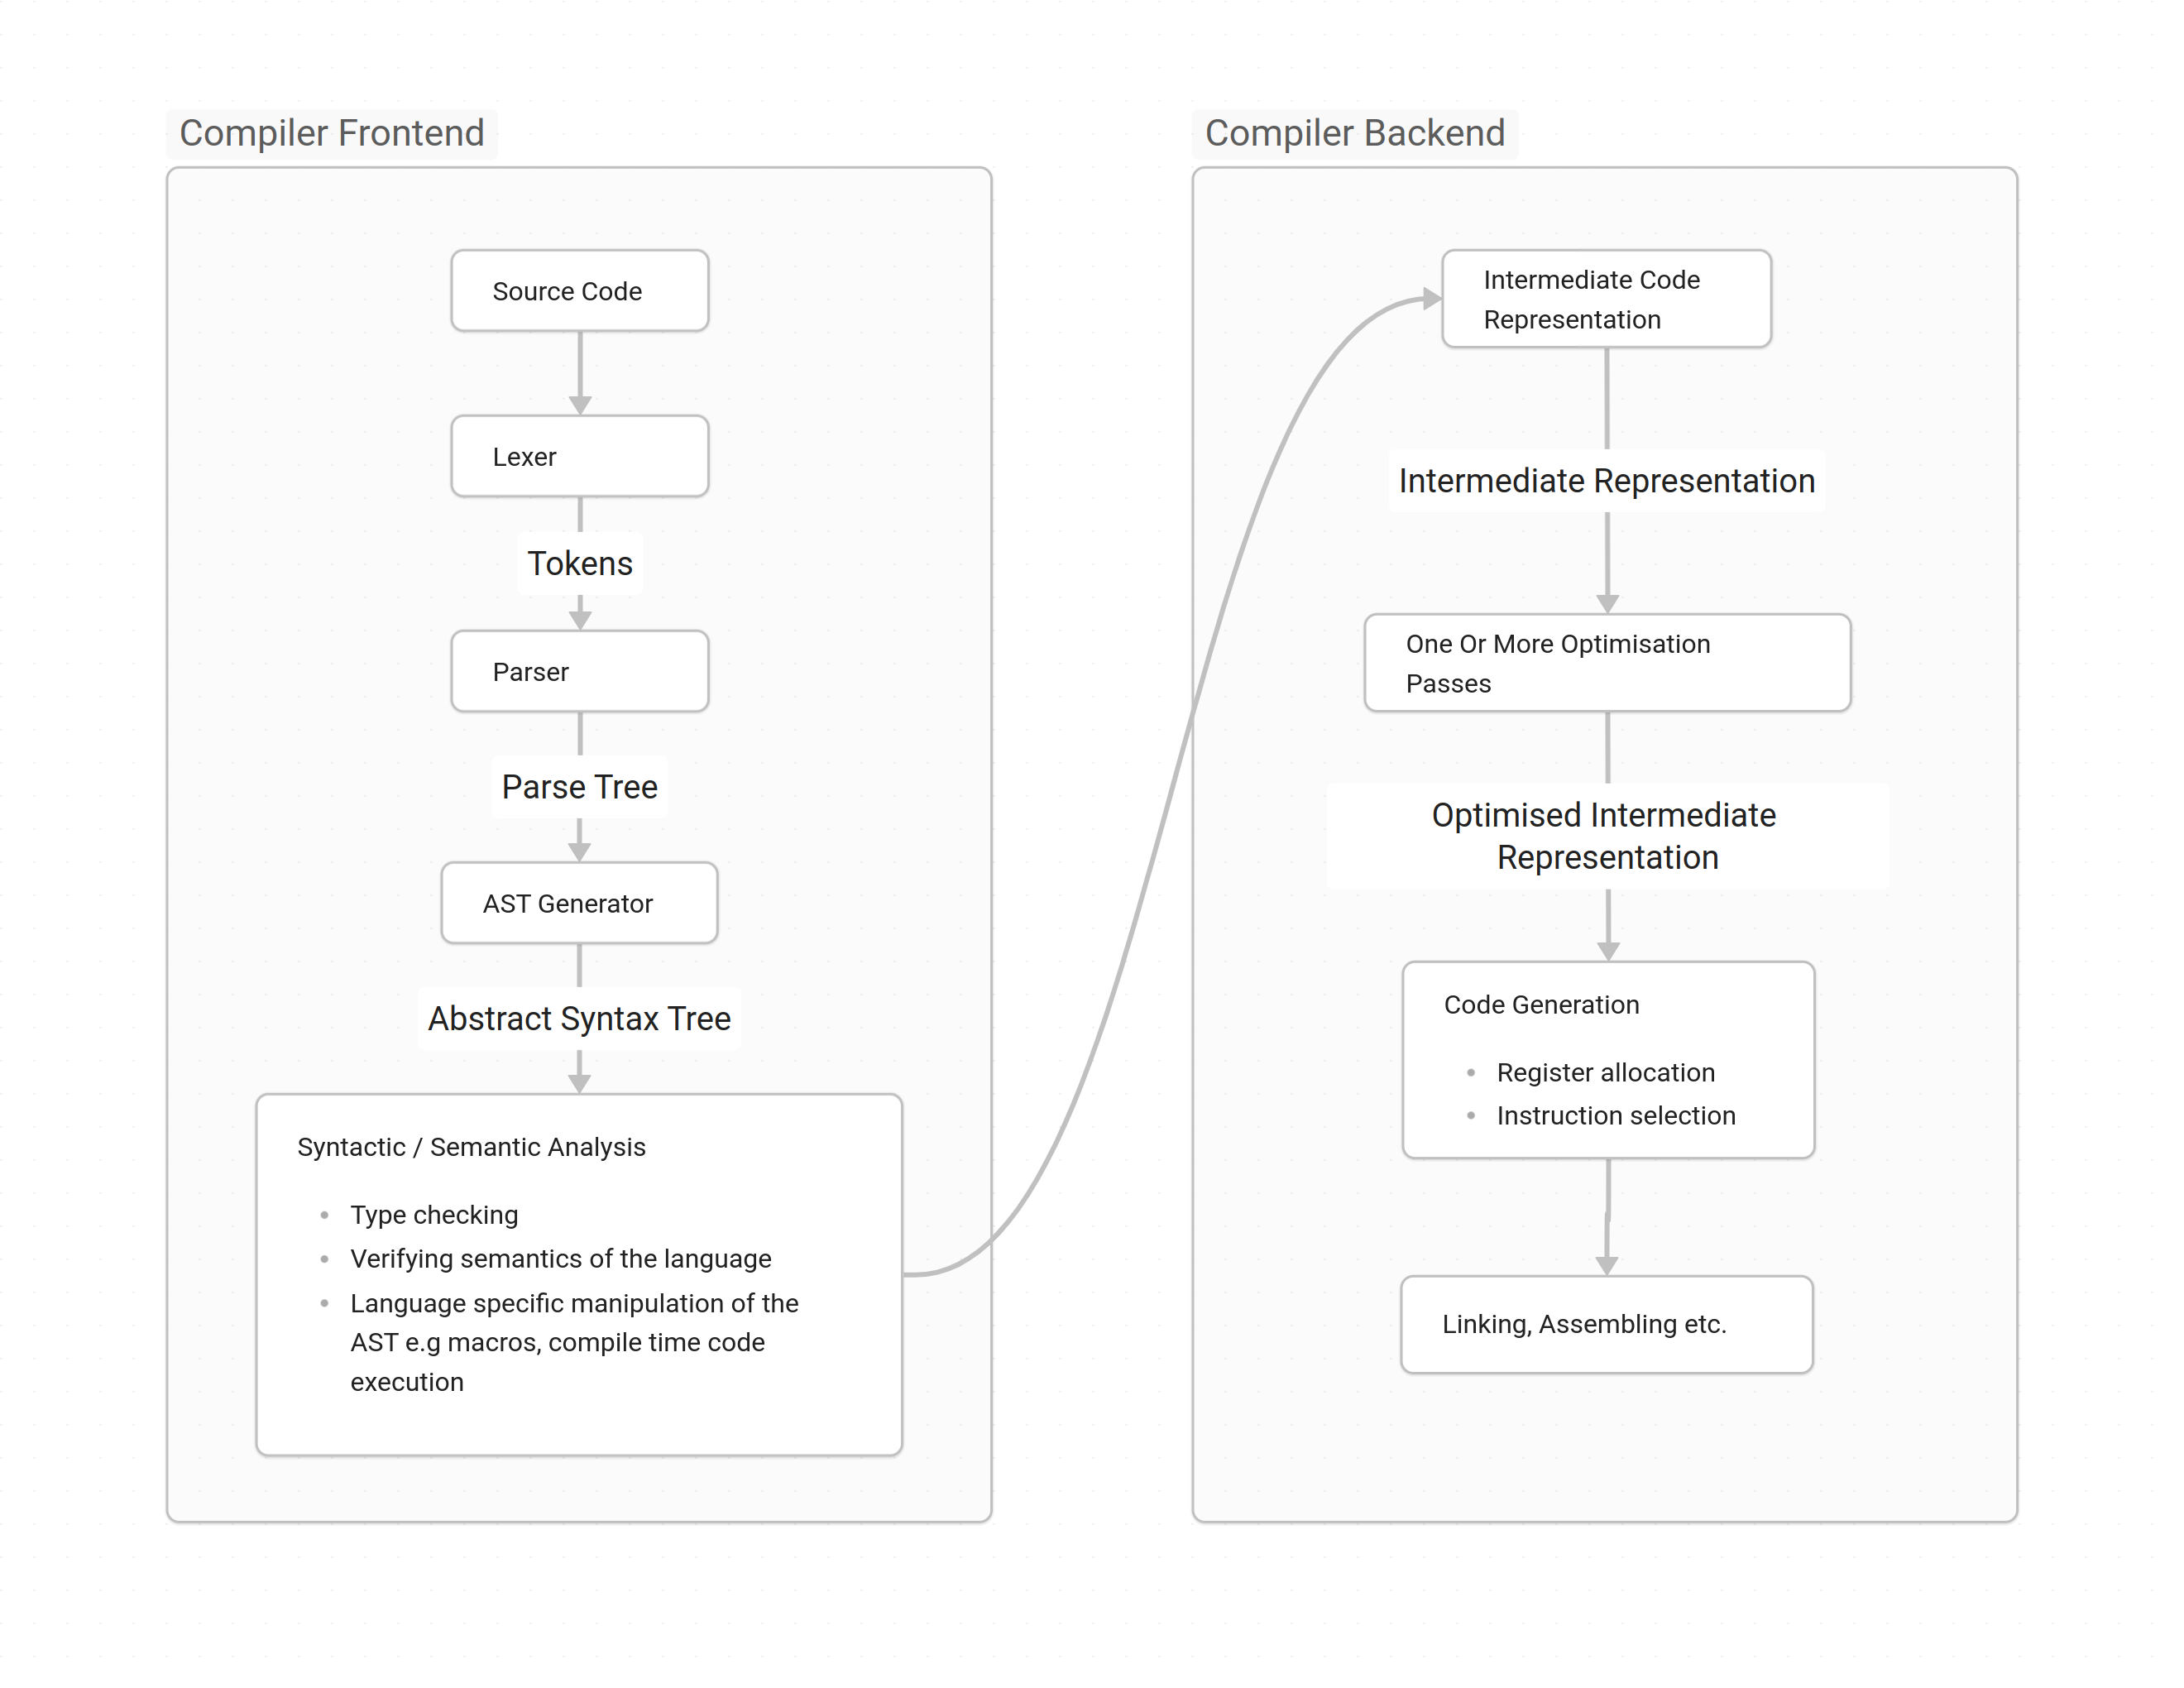
\includegraphics[width=\linewidth]{images/generic_compiler.png}
\centering
\caption{Compilation phases in a generic compiler}
\label{fig:compiler}
\end{figure}

Compilation is the process of translating a program written in a high-level
programming language into a semantically equivalent program written in a
lower-level programming language such as assembly or machine language. During
this process, a compiler will usually lose information in the source code that
is useful to the programmer but is useless to the machine that will ultimately
execute the program. Inside a compiler, the source code passes through several
algorithms that transform the code in various ways. These compilation stages are
shown in Figure \ref{fig:compiler}

The work of a compiler can be described as a multi-stage process resembling a
pipeline, where each stage works on the output of the previous stage thereby
producing the input for the next stage. The lexer splits the source code into
lexemes which are then tokenized for the next stage. In the parser stage, based
on the rules of the source language the code’s syntax is verified. During this
stage, an \gls{ast} is created, reflecting the hierarchy of the elements in the
code such as, tokens, variables and statements, and the relationships between
them. This AST is then analysed during the semantic analysis stage, considering
type checking, variable declaration prior to usage, unused variables and so
forth. The parts of the compiler up to this point are colloquially called the
frontend of the compiler.

These stages of compilation are often executed sequentially with each stage
doing the least amount of work neccessary before passing control to the
subsequent stage. For example, the lexer will do only enough work to retrieve
the next token before passing that token to the parser. The parser will then
begin executing, doing as much work as it can with the input it got from the
lexer. Once it has done that, it might request more tokens from the lexer,
in which case control is returned to the lexer. This process repeats until
the entire contents of the source code in the input file has been processed.
Compiling in this way is much more memory efficient compared to performing
a compilation stage to completion prior to moving onto the next stage.
Difficulties with implementing this architecutre using parallel processing
methods is described in Section \ref{compiler_parallel_methods}.

This type of architecture has traditionally been driven by a need to optimise
for memory use and single threaded performance. For example, in the C
programming language, programmers are forced to declare functions before they
are called. This was originally done to allow the compiler to fully compile
each function independantly, without needing to keep all the other functions
in memory and avoiding a costly second pass over code (\textbf{citation
needed}). As a result of these decisions aswell as historical circumstances,
the stages of a compiler that are reponsible  for taking a file containing
source code to code generation are often implemented with little to no
parallelisation (\textbf{citation needed}). An example of going from source code
to machine code is the process of compiling a C file into an object file. As can
be seen from figure \ref{fig:compiler}, this envelopes a significant portion of
the compiler. The next section describes parallel compilation.

\section{Advantages of Parallel Compilation} \label{advantages_parallel_compilation}
\begin{comment}
\begin{sectionplan}
	What is meant by parallel compilation?

     Reasons why parallel compilation is good / better compared to sequential
	 compilation.

     \begin{itemize}
          \item More cores used during compilation increase compiler performance
                and better overall system usage

          \item Hardware investments in the industry involve specialisation
                and increasing reliance on performance gained from parallel
                architectures. Existing compilers cannot benefit from this.

          \item Choosing a language syntax as a language designer based on how
                well it can be processed in parallel in the future is necessary
                early on. Making those choices is difficult due to a lack of
                research.
     \end{itemize}
\end{sectionplan}
\end{comment}

Parallel compilation uses parallel processing methods in order to perform
various compilation stages at the same time. Parallel processing involves
executing more than one piece of code simulaneously. This can be achieved in
various ways depending on the available hardware. The most common of these
methods are reviewed in Section \ref{parallelisation_methods}. Potential ways
to structure such a compiler that uses such methods is discussed in Section
\ref{compiler_parallel_methods}. This section considers the motivation for
performing various stages of compilation in parallel.

\subsection{Increased Compilation Speed with Additional Cores}

Using multiple \gls{cpu} cores during compilation can signficantly speed
up compilation time. IBM researchers created an optimised lexer for a
machine that had a large number of cores that could run code in parallel
\citep{scarpazza_high-performance_2009}. It had eight \gls{cpu} cores where each
core could run eight threads in parallel for a total of 64 parallel threads.
More recent research into parallel lexing from 2014 achieved a 14 times speed
up for lexing HTML on a 16 core system \citep{mytkowicz_data-parallel_2014}.
Substantial performance gains can clearly be achieved through parallelisation.
This shows how using parallel processing to speed up compilation tasks is not a
new idea.

\subsection{Parallel Compilation Research Aids Language Design}

For several programming languages, once their syntax goes into general use, it
becomes nearly impossible to reverse or change it, without breaking programs
already written in the particular language. This leads to programming languages
becoming complicated and difficult to define as new features are added. For
example, langauges like C++ are very difficult to compile in a sequential
manner, let alone in a parallel manner (\textbf{citation needed}). Research into
and the development of parallel compilers can aid future developers when they
are choosing their syntax or what features they want to implement without making
their language difficult to compile in parallel (\textbf{citation needed}). It
is currently rather difficult to design a language that can easily be compiled
in parallel due to a lack of research and prior work as compared to sequential
approaches (\textbf{citation needed}).

\section{Advantages of Data-Parallel Compilation} \label{advantages_of_data_p_comp}
\begin{comment}
\begin{sectionplan}
	Justify looking at alternative forms of parallelism besides the status quo 	
	method of compiling source files in parallel and linking them together in the
	end.

	\begin{itemize}
     	\item Finer grained parallelism is better suited for running code on 				
			  massively parallel hardware like GPU's.

     	\item Error handling potential improved by being able to independantly
			  process any part of text. No need for complex parser recovery.

     	\item More parts of a program can be compiled in parallel which makes
			  better use of a computers parallel processing facilities. Mention 
			  ahmdals law.

		\item Significant speedups in other fields where only one stage of is 
			  needed like lexing and parsing very large amounts of structured 
			  data. Mention PAPAGENO parser with relation to simdjson.
	\end{itemize}
\end{sectionplan}
\end{comment}

Several current compilers can operate in parallel by compiling several source
code files at the same time. In this work I am looking at methods employing
\gls{data_parallel} techinques where various stages of a compiler can be executed in
parallel when compiling the same file. Due to a lack of prior work comparing
the two approaches directly, it is difficult to make an objective statement
regarding which approach is better. I will instead focus on the potential
advantages and disadvantages of using such a finer-grained approach.

\subsection{Parser Error Recovery}

An important responsiblity of a compiler is to detect syntax errors and
present useful error messages to the programmer. Such syntax errors are often
detected during the parsing stage. An issue arises when a parser must then try
to continue parsing after encountering a syntax error. This parser recovery
process is frequently complicated and sub optimal \citep{medeiros_syntax_2018,
hutchison_pika_2020}. Certain parallel parsing algorithms, such as those
described in \citet{clarke_error_1993} and \cite{barenghi_parallel_2015}, allow
a compiler to forgo a complicated parsing recovery process by being able to
restart the parsing process immediately after encountering an error.

\subsection{Applications in Massively Parallel Computing}

There have been increasingly larger investments in the hardware industry for
specialised hardware beyond the typical \gls{cpu}.  For example, smart \gls{nic}
s that offload network packet parsing from the \gls{cpu} or \gls{dpu} to provide
more facilities for networking and input/ output related tasks than a typical
\gls{cpu}. A recent article from October 2023 outlined how the software stack
of \gls{amd} for general purpose computing on graphics cards known as \gls{rocm}
is now among their top priorities \citep{ward-foxton_rocm_2023}. As time goes
on, we are likely to see increasingly specialised and heterogenous hardware
(\textbf{citation needed}).

Current compilation algorithms scale poorly on massively parallel hardware
such as \glspl{gpu}s. This is due to the restrictions imposed on programs by
computing in such an environment. An approach utilising \gls{data_parallel}
data structures described by \cite{hillis_data_1986} was applied by
\cite{voetter_compilation_2022} in order to create a parallel compiler
implementation that could run on a \gls{gpu}. This shows how  re-architecting
the compilation process makes it possible to execute a compiler in a massively
parallel environment, potentially achieving a linear performance increase that
scales with the number of available processing cores. This can only be achieved
by efficiently using \gls{data_parallel} techniques.

\subsection{Increased Performance in Individual Compilation Stages}

Data parallelism can massively improve the performance of various workloads
that utilise individual compilation stages. Tasks that involve processing large
amounts of data benefit the most. \cite{barenghi_parallel_2015} demonstrated
how \gls{json} parsing can be performed much faster using a parallel parser.
\cite{mytkowicz_data-parallel_2014} optimised a parallel regular expression
matching algorithm which has a large number of uses beyond lexical analysis.

\section{Project Objectives}

The goal of my \gls{fyp} is to research methods and algorithms for use in the stages
of a parallel compiler frontend and to justify the selection of those included
in the implementation of same.

\section{Structure of Report} \label{structure_of_report}

Chapter \ref{introduction} provides an introduction to compilers as well as
reasons to study parallel compilation methods.
\newline \newline
Chapter \ref{litreview} describes approaches for compiling
in parallel.
\newline \newline
Chapter \ref{design} will elaborate on the issues associated with designing a
parallel compiler, presenting suggested approaches from literature to overcome
these, prior to focusing on the compiler design and implementation decisions
specific to this work.
\newline \newline
Chapter \ref{implementation} explains the details of my implementation,
referring to aspects such as external code dependancies and program structure.
\newline \newline
Chapter \ref{evalandtesting} describes my testing methodologies and the
evaluation of my compilers performance.
\newline \newline
Chapter \ref{conclusion} concludes the report with a summary of the report and
concluding remarks.

\newpage
\chapter{Literature Review} \label{litreview}

In this literature review I research techniques for creating a parallel
compiler. This review has helped me to develop a better understanding of how
parallel compilers work and how to approach implementing one. Time constraints
make it impossible to review all literature on the topic however
an attempt is made to cover important developments in parallel compilation
research.
\newline \newline
Section \ref{parallelisation_methods} describes hardware capable of executing
code in parallel.
\newline \newline
Section \ref{compiler_parallel_methods} describes different ways of designing a
compiler such that parts of it can be executed simultaneously.
\newline \newline
Section \ref{lit_review_lexing} describes various algorithms to perform lexing
in parallel.
\newline \newline
Section \ref{lit_review_parsing} describes various algorithms to perform parsing
in parallel.
\newline \newline
% Section \ref{lit_review_analysis} describes various algorithms to perform semantic
% analysis in parallel.
% \newline \newline

\section{Parallelization Methods} \label{parallelisation_methods}
This section describes various hardware solutions for executing code in
parallel. Parallel processing methods can strongly impact the performance
for a parallel program as well as the complexity of its implementation. This
makes it worthwhile to research and analyse various forms of parallelization
in order to make informed decisions about how they will be used in the final
implementation.
\newline \newline
Section \ref{simd} describes \gls{simd} instructions which are used to implement
instruction-level parallelism.
\newline \newline
Section \ref{multithreading} describes a more granular form of parallelization
called multi-threading or multiprocessing.
\newline \newline
Section \ref{gpgpu} describes highly parallel computing on graphics cards.

\subsection{Single Instruction Multiple Data} \label{simd}

\gls{simd} instructions are assembly instructions that can process more data
than a typical assembly instruction. Instead of processing data with normal
registers, \gls{simd} instructions use special registers that are several
times larger than normal registers. This allows a processor to compute an
assembly instruction over parts of the register in parallel. These instructions
are also known as vector instructions since they process lists or vectors
of data. As an example, in the Advanced RISC Machines (ARM) instruction
set, the ADD instructions can be contrasted with its corresponding vector
instruction UQADD8 which adds four 8-bit numbers with four other 8-bit numbers
\citep{noauthor_arm_nodate}.

Since vector instructions are functionally similar to a collection of assembly
instructions being executed simultaneously, a program written using vector
instructions can be similar in structure to an equivalent sequential one. This
makes it possible for compilers to automatically utilize these instructions
to speed up existing sequential programs in a process called vectorization.
Vector instructions can also be manually written by the programmer in order to
improve performance \cite{langdale_parsing_2019, mytkowicz_data-parallel_2014}.
Although using vector instructions can be significantly faster than the
sequential case, this performance benefit is only up to a point. Increasing
performance past a certain threshold requires larger registers which take a
long time to architect and standardize in a \gls{cpu}. The methods described in
Section \ref{multithreading} scale better at the cost of having a more complex
implementation.

\subsection{Multithreading/Multiprocessing} \label{multithreading}

Multicore parallelism makes it possible to have multiple programs execute
at the same time through the multi-threading facilities exposed by most
modern \glspl{cpu}. Each process can have its own call stack and its own view
of memory. This freedom in program execution and memory access allows for
performant designs of complex parallel algorithms. The performance of a well
implemented program can potentially scale with the number of \gls{cpu} cores
available to the program. For example, if a parallel program can run in one second
on one thread then in it should run in a quarter of a second on four threads. In
reality, there is overhead from thread creation, synchronization and management
that prevents a perfectly linear performance improvement.

The downside of multithreading is the difficulty in creating reliable, bug free
programs.  This processing model adds new classes of bugs, such as data races
that can occur in shared memory scenarios.  When converting a sequential program
to a multithreaded one, it is usually necessary to re-architect significant
portions of it in order to better fit this processing model. Furthermore,
managing shared memory is difficult and can lead to subtle yet complex bugs.

\subsection{General Purpose Computing on GPUs} \label{gpgpu}

It is possible to use graphics cards for general purpose computing, called
\glspl{gpgpu}. It is conceptually like programming a specialized \gls{cpu} that
has hundreds if not thousands of cores. Programming for a \gls{gpu} requires
a programmer to significantly re-architect a program in order to fit the
\gls{gpu} programming model. There are additional issues, such as the time it
takes to compile \gls{gpu} programs and the large latency between a \gls{gpu}
and main memory. In fact, this latency can be so large that processing small
amounts of data can be much less performant than a single-threaded \gls{cpu}
implementation. In general, large scale computing on a \gls{gpu} can be
strongly worthwhile if program can operate within the constraints of a \gls{gpu}
environment. 

\section{Methods of Parallelizing A Compiler} \label{compiler_parallel_methods}

\cite{gross_parallel_1989} outline three key approaches for parallelizing a
compiler. The first approach consists of splitting the source code of a program
into chunks and processing each chunk individually. Many compilers divide up
source code at the filesystem-level where each file of source code can be
compiled separately from other parts of the program. Although this approach is
already somewhat \gls{data_parallel}, it can be taken even further where each
file is split into even smaller chunks, with each of these chunks being
processed independently.

The second approach is termed computation partitioning. This is described as
a series of sequential computations that can be divided up and processed in
parallel with the results of each computation being joined together at the end.

The final method is pipeling which involves dividing a computation into some
number of phases where each phase depends on the output from the previous phase.

\cite{mark_thierry_vandevoorde_parallel_1988} attempts to implement a parallel
C compiler using a \gls{data_parallel} approach with a traditional a two-pass
compiler architecture.

\section{Lexing} \label{lit_review_lexing}

\cite{scott_programming_2015} describes lexing as the process of removing
unnecessary characters from source code and grouping characters of interest
together into lexemes. This compilation stage emits a list of lexemes that are
later passed to the parser. The purpose of lexing is to simplify the task
of the parser by reducing the size of its input. Lexing is sometimes  called
tokenization or lexical analysis and it is performed by a lexer, sometimes
called a tokenizer or lexical analyser. Lexers are defined using \glspl{reg_exp}
that describe the character sequences which need to be found and emitted from
the lexer as lexemes. Since \glspl{reg_exp} can be described as a \gls{fsm}, a
lexer can similarly be described as one.

A \gls{fsm} is a model of an abstract machine that can be in one of a finite
number of states at any given time. A \gls{fsm} works by accepting input symbols
which can cause the state of the \gls{fsm} to change according to a set of
state transition rules that define the \gls{fsm}. A \gls{fsm} can be described
as either a \gls{nfa} or as a \gls{dfa}. In a parallel lexer where the output
in one thread may depend on the output of another thread, it is undesirable to
have different results based on the same input because it can lead to bugs and
an unpredictable output. This situation can occur in a \gls{nfa} which makes
it non-trivial to design a parallel lexer around \gls{nfa}. The deterministic
property of a \gls{dfa} ensures that the resulting state of a
\gls{dfa} will always be the same for a given input.  As such, structuring a
lexer as a \gls{dfa} can ensure a consistent and repeatable computation for a
given chunk of source code.

A common approach to multithreaded lexing involves structuring the lexer as a
\gls{dfa}, splitting the input into some number of parts, lexing each part on
its own thread and joining up the results at the end. Due to the inherent data
dependency between state transitions in a \gls{dfa}, the initial state for a
chunk of code depends on the output computed from lexing the code just before
it. This causes the issue of determining the initial start state of all the
lexers besides the one computing the first part of the overall input. A solution
to this problem is through speculative simulation where an algorithm speculates
on the unkown initial states of these \gls{dfa}s.

\subsection{Simulation of DFA} \label{simulation_of_dfa}

One approach to speculative simulation is the brute force method of computing
a \gls{dfa} for every possible state it can be initialized with. Such a
lexer begins by splitting its input into chunks and processing each chunk
independently on a separate thread. Once all threads are finished lexing,
the outputs from each thread are checked, starting from the first chunk of
code, such that the finishing state of the lexer corresponds to the initial
state of the lexer that computed the subsequent chunk of code. The correctness
of computing a \gls{dfa} in this way relies on the  associativity of state
transition functions as described in the parallel prefix sum algorithm in
\cite{hillis_data_1986}. This algorithm is explained more formally with both a
message passing and a shared memory implementation by \cite{holub_parallel_2009}
and a variation of it in a cloud computing environment is shown by
\cite{ko_speculative_2012}. The need to compute the output for every possible
initial state can result in many unnecessary computations which can
significantly impact performance for \glspl{dfa} with many states.

\cite{barenghi_parallel_2015} optimize this by using a heuristic where the
source code is split into chunks that start with symbols that have known and
consistent initial states. These symbols are found by scanning ahead when the
source code is being split until such a symbol is found. The symbols that a
chunk of code can start with are language dependant. If a symbol is allowed to
appear in a lexeme, such a string or comment, then multiple initial states must
be additionally computed.

Instead of using a language specific heuristic,
\cite{mytkowicz_data-parallel_2014} attempted to optimize speculative simulation for
any given \gls{dfa}. The core algorithm is very similar to the one previously
described. It begins with the assumption of needing to compute the \gls{dfa} for
every possible initial state the input can be in. Instead of using a language
specific heuristic like \cite{barenghi_parallel_2015}, which is determined ahead
of time, \cite{mytkowicz_data-parallel_2014} define a convergence algorithm
which reduces the number of states that need to be computed at runtime. It
follows from the observation that many states transition to the same state on
a given input symbol. Once this convergence of state occurs, looking up the
state transition for each state becomes redundant as it is going to be the same
for subsequent input symbols. By factoring out these common states, the number
of actual state transitions that need to be computed drops significantly for
most \gls{dfa}s, especially structured and non-adversarial ones. Heuristics
are used to determine when to check for a  convergence of states. The previous
heuristic as well as this convergence algorithm are similar in some ways however
the solution proposed by \cite{mytkowicz_data-parallel_2014} is more generally
applicable by not being tied to a specific language.

\cite{mytkowicz_data-parallel_2014} additionally utilize \gls{simd} instructions
in order to perform the state transitions for a given transition function
and set of states. This parallelizes an important part of the algorithm and
significantly improves performance. A technique called range coalescing is also
used to reduce the number of memory addresses accessed when computing state
transitions for many states. \cite{zhao_--fly_2015} implement a convergence
algorthim similar to the one described by \cite{mytkowicz_data-parallel_2014}.

\subsection{Speculative Simulation} \label{speculative_simulation}

Another method is speculative simulation which attempts to simply guess the
initial state of the \gls{dfa}s, possibly with a way to back track or validate
its result in case of an incorrect guess. \cite{luchaup_multi-byte_2009,
luchaup_speculative_2011} implements a speculative method which simply guesses
the unknown initial \gls{dfa} state. This optimization works due to its specifc
use in intrusion detection systems where a \gls{dfa} spends most of its time
in a small number of states which can be guessed with sufficient accuracy to
outweigh the cost of validation in case of failure.

\subsection{Prescanning} \label{lit_prescanning}

\cite{bernecky_spmdsimd_2003} describes a multi-pass parallel APL tokenizer
written in APL which performs several scanning phases in order to pre-process
source code as well as find strings, comments and identifiers, among other
tokens, in distinct passes over the source code. It is not table driven and is
instead specialized for APL. Since the computational complexity of the compiler
is high and its performance is not evaluated by the authors, it remains unknown
if it is an improved approach to parallel lexing.

A variation of the heuristic approach by \cite{barenghi_parallel_2015} is
implemented by \cite{li_plex_2021} that generalizes it and makes it language
independent. It builds on work from \cite{sinya_simultaneous_2013} and
\cite{zhao_--fly_2015} to perform a pre-scanning phase by generating and
executing a \gls{dfa} based on the lexical grammar that determines the context
for \glspl{dfa} in a subsequent tokenization phase.


% \subsection{Other Approaches} \label{other_approaches}

\begin{comment}
\cite{sinya_simultaneous_2013} propose a novel type of finite automata called
\gls{sfa}.
\newline \newline
Mention \cite{lin_accelerating_2013, wang_hyperscan_2019,
li_plex_2021, asthagiri_associative_1992} Go and look at references cited in
\cite{zhao_--fly_2015}
\newline \newline
Could mention these but the fella doesn't do anything novel (and his
grammar is questionable) \cite{barve_parallel_2014, barve_parallel_2012,
barve_improved_2015}
\end{comment}

\section{Parsing} \label{lit_review_parsing}

Parsing is the second canonical stage of a compiler. The goal of a parser
is to take a list of lexemes from a lexer and structure them as a graph
\citep{scott_programming_2015}. This structure makes it easier to navigate
and manipulate the source code using concepts defined by the language like
variables, functions and control structures. The graph structure created by
a parser is typically called a syntax tree or a parse tree. It is created
according to a parsing grammar that defines how it should be built. The rules
of a parsing grammar that govern how lexemes should be processed in order to
validate an instance of the language and build a parse tree representing it
are called production rules. A parser might additionally process a parse tree
as it is getting built, or during a separate subsequent processing step, which
produces an \gls{ast}. This data structure is later analysed during the semantic
analysis phase. There exist different families of parsers that group parsers by
similarities in their method of parsing.

\gls{ll} parsers read the source code from left to right and construct a parse
tree from the root node down, predicting at each step which production will be
used to expand the current node, based on the next available token of input.
\gls{ll} parsers are also called recursive descent parsers due to their typical
implementation of recursively calling a function for every non-terminal in a
production. Many modern compilers use recursive descent parsers because they
can easily be implemented by hand and make it is easier to generate good error
messages for the user. An alternative approach is to create an \gls{ll} parse
table for a given grammar and use a driver program that parses tokens according
to the rules stored in the parsing table. A program that uses this table to
generate and output source code for a recursive descent parser is a parser
generator.

In \gls{lr} parsing, source code is read left to right but the parse tree is
constructed by first creating the leaf nodes and later grouping these nodes
together into trees. This kind of parser works by maintaining a stack of tokens
and parse tree nodes during parsing. The parser will match this list against
the right side of the grammars production rules. If a match occurs, the tokens
on the stack become children of a new node corresponding the left side of rule.
This new node, corresponding to a subtree of the final parse tree, is pushed
onto the stack. Parsing finishes once the root node (axiom) is built from the
nodes on the stack. This type of parser is also called a shift-reduce parser due
to its two main operations, shifting tokens on the stack and reducing them into
new parse tree nodes.

\gls{ll}($k$) and \gls{lr}($k$) denotes how many tokens these parsers must look
ahead in the input in order to resolve ambiguities between production rules.

\subsection{Parallel LR Parsing} \label{parallel_lr_parsing}

\cite{barenghi_parallel_2015} proposes and implements a non-speculative \gls{lr}
(0) parallel parser generator for \gls{opg}s. A key insight is in constraining
the grammar sufficiently such that it can be deterministically decided whether
a string of bounded length contains the right-hand side of a production
and can be unequivocally replaced by its corresponding left-hand side. This
is in contrast to other approaches that require the parser to speculate on
possible production rules in order to reduce them when parsing in parallel
\citep{mickunas_parallel_1978}.

\cite{li_associative_2023} builds on the work by \cite{barenghi_parallel_2015}
and optimizes the parser for a common case encountered in real word data. When
parsing a long list described by a recursive production rule, the whole list
must be parsed in order to reduce it into a parse tree node. This means that
if the list is large enough to be parsed by multiple threads then the final
operation which reduces the stack will be deferred until all the threads have
finished. Moreover, if there is little work for the parser to do per element
in the list, then the bulk of the parsing will be left until the final joining
phase of the parser. The contribution from \cite{li_associative_2023} is a way
of recognizing operators in the grammar that are associative so that elements of
such lists can be more effectively reduced into parse tree nodes before knowing
they are part of a list.


\subsection{Parallel LL Parsing} \label{parallel_ll_parsing}

\cite{vagner_parallel_2007} A deterministic parallel LL parsing algorithm is
presented. The algorithm is based on a transformation from a parsing problem to
parallel reduction. First, a nondeterministic version of a parallel LL parser
is introduced. Then, it is transformed into the deterministic version — the
LLP parser. The deterministic LLP(q, k) parser uses two kinds of information to
select the next operation — a lookahead string of length up to k symbols and a
lookback string of length up to q symbols. Deterministic parsing is available
for LLP grammars, a subclass of LL grammars. Since the pre- sented deterministic
and nondeterministic parallel parsers are both based on parallel reduction, they
are suitable for most parallel architectures.

\cite{mark_thierry_vandevoorde_parallel_1988} exploits C's syntax and semantics
by forking his recursive descent parser (an \gls{ll} parser) in places where
the code under parse does not depend on the code surrounding it. 

\cite{skrzypczak_parallel_2012} Implments a \gls{cpu} and \gls{gpu}
implementation of the CYK parsing algorithm.

\section{Semantic Analysis} \label{lit_review_analysis}

Semantic analysis is the third stage canonical stage of compilation. The goal of
this stage is to analyze the output from the parser to see whether it conforms
to  the semantic rules that define the language. Informally, parsing attempts
to find the structure of a program whereas semantic analysis tries to find its
meaning. 

\cite{seshadri_investigation_1991} implements a parallel semantic analyzer for
a regular, block structured language. It checks whether variables have been
declared before being used. The \gls{dky} problem is introduced which describes
the issues with analyzing code without full context. The \gls{dky} problem is
encountered when the analysis process is performed somewhere within the code
and it isn't yet known whether a variable has been declared. The authors then
propose three approaches to avoid or minimize its impact.

\begin{enumerate}
    \item DKY Avoidance - involves scheduling processes in the compiler in
order to avoid DKYs during semantic analysis. This technique was also used by
\cite{gross_parallel_1989}.
    \item DKY Handling
    \item Two part DKY Handling
\end{enumerate}


\section{Conclusion}

My 

\subsection{Parallelization Method} \label{design_parallel_method}

When designing a parallel compiler, one must first choose an appropriate
paralleization method. This decision is important because it can impact the
performance of the compiler, as well as the programming language and algorithms
used in its implementation. For this project I considered between using the
parallel facilities of GPUs, multicore CPU's and SIMD capable CPU's. There exist
other ways of executing code in parallel however those methods were unavailable
at the time of writing.

Computing on the GPU affords the highest peak performance due to being built
with data-parallism in mind. Unfortunately, however, programming on a GPU is
difficult, running small tasks on it is impractical and trying to create a
compiler that runs on the GPU requires making big concessions in regard to the
compiler architecture and language design. Although promising results were shown
by \cite{skrzypczak_parallel_2012}, even for input as small as 200 lexemes,
other work such as that by \cite{voetter_compilation_2022} shows very large
overhead for average sized inputs. Due to these issues I determined that writing
a parallel compiler frontend to work on the GPU would be impractical.

On the other hand, multicore parallelism is much more flexible and commonly
available. 


\subsection{Lexer} \label{lexer}

The core issue with parallel lexing is figuring out the inital state
of the \gls{fsm} for all but the \gls{fsm} processing the first chunk of
input. This can be solved through enumerating through all possible initial
states or simply guessing the most likely state and backtracking if guessed
incorrectly. Speculative approaches that guess the initial \gls{fsm} states
can be effective, as shown by \cite{luchaup_speculative_2011}, however
\cite{mytkowicz_data-parallel_2014} points out two major issues that can
arise. The efficacy of the speculative approach is difficult to predict and
it is limited by the sequential implementation on a single core. In contrast,
enumerating through all possible inital states is predictable against even
randomly generated input and can benefit from fine-grained parallelism afforded
by a single core.

For my implementation I've chosen to use the enumerative approach where I will
enumerate over all possible initial states for the \glspl{fsm}. I hope this will
lead to a more robust system that is resistant to edge cases and adversarial
input. Although I initially aim to create a handwritten lexer that works in
parallel, I hope to create a table driven lexer if time allows. This will help
me in quickly iterating over the lexical grammar to better fit the parsing
grammar.

\subsection{Parser} \label{parser}

There are many parser designs available in the literature. The one I have chosen
is the \gls{opg} parser by \cite{barenghi_parallel_2015}. It has a simple design
that allows for a straightforward implementation. 

\subsection{Semantic Analyzer} \label{parser}

For this compilation stage I intend to create my own algorithm for finding if
all variables had been declared before use.


\newpage
\chapter{Design} \label{design}

\section{Lexer}
\begin{itemize}
	\item Lexical grammar, defined with regex's and parsed with regex syntax crate.
	\item Use that to create NFA graph using Thompson's construction.
	\item Convert the NFA into a DFA using powerset construction.
	\item Generate a state transition table by traversing the graph.
	\item During generation, look for duplicate state transitions where the
		  characters are the same, but states differ. This indicates that those
		  states are potential start states of the lexer.
	\item Split up the source code into n chunks and put them onto a work queue.
	\item These chunks are taken off the work queue by a thread pool. Each chunk
		  is lexed for each possible start state, resulting in n number of outputs for n
		  number of start states, per chunk.
	\item 
	Once all chunks have been processed, the correct output from each chunk is
		  chosen such that its start state is the same as the previous chunk's finish
    	  state. Remaining outputs are discarded.
\end{itemize}

The goal of a lexer is to recognise patterns in text and emit lexemes associated
with these patterns. For this purpose I decided to use regular expressions as they 
are expressive

\begin{comment}
Insert a figure here like the one in data-parallel finite state machines.
\end{comment}

\begin{enumerate}
	\item 
\end{enumerate}

The first step of the lexer is to create a state transition table from a
lexical grammar. A lexical grammar is defined as a mapping between lexemes and
regular expressions. The lexer should output a lexeme if the regular expression
associated with it is encountered in the source code. In order to tokenize the source code 


	\item Split the source code into many parts and tokenize each part using the
		  state transition table from the previous step.
	\item Once all parts have been processed, the correct output from each chunk is
		  chosen such that its start state is the same as the previous chunk's finish
    	  state. Remaining outputs are discarded.
\end{enumerate}



The goal of the lexer is to use this lexical grammar
in order to generate a state transition table that can be used


\section{Parser}
\begin{itemize}
	\item Read grammar from file that defines terminals, non-terminals nad production rules.
	\item Transform grammar into floyd normal form as defined in \cite{barenghi_parallel_2015}
	\item Build operator precedence table according to \cite{grune_parsing_2008}
	\item Take the lexer output from the previous step and parse each chunk using the same
  		  thread pool approach. The parsing algorithm returns a partial parse tree and a stack of lexemes.
	\item Take the outputs from each chunks and join the paritial parse trees using
  		  the same parsing algorithm.
\end{itemize}

\section{Semantic Analysis}
\begin{itemize}
	\item Iterate over the parse tree in post-order DFS in order to generate the Abstract syntax tree.
	\item Iterate over AST using pre-order DFS, creating a new thread and symbol table for certain nodes.
	\item Check if variables are defined before they are used by checking if they exist in ancestor symbol tables.
\end{itemize}



\newpage
\chapter{Implementation} \label{implementation}

For this project I implemented the design as described in the previous chapter.
It is a command line application that takes a source code file as input and
performs semantic analysis on its \gls{ast}. I chose to write my implementation
using the Rust programming language. It is a memory safe language that leverages
the LLVM backend for highly optimized code. This makes it easy to write
robust and performant code. It additionally has very good parallel programming
facilities and an extensive software ecosystem that makes it ideal for this kind
of project. 

\begin{listing}[t]
\begin{minted}[linenos]{text}
fn factorial[n: int] {
    if n == 0 {
        return 1;
    } 

    return (n * factorial(n - 1));
}
\end{minted}
\caption{Factorial in the test language.}
\label{lst:factorial_example}
\end{listing}

Due to a generic lexical and syntatic analysis implementation, as described in the previous chapter,
the compiler supports parsing JSON aswell as a bespoke test language with syntax similar to Rust,
shown in Listing \ref{lst:factorial_example} and \ref{lst:json_example}.

Section \ref{structure} provides an explanation of the programs structure as well as some
implementation details.
\newline \newline
Section \ref{test_lang} discuss the some additional, language specific code that was needed in order
to support \gls{json} and the test langauge.
\newline \newline
Section \ref{dependancies} concludes with a description of the projects dependancies and their
purpose in the implementation.

\section{Structure} \label{structure}

I will explain the implemention in the order of its execution. The program is divided into three
general stages: lexical, syntactic and semantic analysis. Each stage is implemeted just it was
described in the design chapter. There are significant pre-processing steps that need to happen
prior to the core lexing and parsing algorithms, which can be computed at compile time, but I
nevertheless chose to do at runtime. The following section begins by describing this pre-processing
work that initializes key datastructures that are used later in the compiler. The subsequent two
sections describe some implementation details of each of the compilation stages.

\subsection{Lexer Preprocessing} \label{lexer_preprocessing}

In order for the compiler to support different languages, while sharing as much code as possible,
it is neccessary to generate datastructures that can be used by a generic lexer and parser.
Furthermore, the datastructures required for bottom-up parsing are very difficult to create without
some form for automatic generation. Although a hand-written, language specific implementation
has significant optimisation potential, as shown by \cite{langdale_parsing_2019}, the focus of my
implementation is to demonstrate the effectiveness of data-parallel compilation. Single threaded
optimisations that leverage the language or \gls{simd} instructions are sufficiently orthogonal to
this goal to put them outside the scope of the FYP.

In order to for the lexer to work, a state transition table must be obtained. This is done by
reading a file that contains the mapping between the lexemes and their corresponding regular
expressions. An example of the syntax can be seen in listing \ref{lst:json_lexical_grammar}. The
\gls{ast} of each regular expression is then traversed and converted into one, large joint \gls{nfa}
graph using thompson's construction algorithm. This is a classic algorithm that is described by
\cite{aho_compilers_2006}, originally attributed to Ken Thompson. It works by recursively breaking
down the regex into simpler components and building an \gls{nfa} for each component. The resulting
NFA recognizes the same language as the original regex. For my implementation I use an external
library to parse the regex into an \gls{ast}. I then traverse this \gls{ast}, building the \gls{nfa}
as described by the algorithm

This graph is then turned into a \gls{dfa} through powerset construction. For this
algorithm I followed the steps outlined in wikipedia article on powerset construction
\citep{noauthor_powerset_2023}. It works by simulating an \gls{nfa} and interpreting the sets of
states reachable from each state in the \gls{nfa}, as the states of the \gls{dfa}. In other words,
it neccessary to simulate the \gls{nfa} and keep track of all states that the automaton could
reach after seeing an input, according to its nondeterministic choices. Each set of choices is then
converted into a corresponding state in the \gls{dfa}.

An example \gls{nfa} and \gls{dfa} for the JSON grammar is shown in figure \ref{fig:nfa} and figure
\ref{fig:dfa}, respectively. I implemented the graph traversals in both algorithms by keeping track
of a stack of nodes that have already been previously encountered. The \gls{dfa} can be tivially
turned into a state transition table by traversing it from its initial state and  taking note of
each pair of states connected by a transition. The parser similarly requires an operator precedence
table that must be computer generated due to its complexity.

\begin{listing}[t]
\begin{minted}[linenos]{json}
{
  "a": 100,
  "b": {
    "x": [
      100,
      "a"
    ]
  }
}
\end{minted}
\caption{Example of parsable JSON.}
\hrulefill
\label{lst:json_example}
\end{listing}

\subsection{Parser Preprocessing} 

The parser defined by \cite{barenghi_parallel_2015} is a standard operator precedence algorithm that
is modified to allow the parsing of non-terminals. This parser requires that the structure of the
language grammar follow certain rules, as been defined in section \ref{design_parser}. A preliminary
validation of the grammar is performed to ensure that it conforms to these rules. This step also
fixes any production rules with duplicate right-hand sides by creating new production rules with
new non-terminals in a way that keeps the resulting parse tree predictable. After this validation
step, the grammar is ready to be used in the parser. Using this grammar an operator precedence
table can be generated by iterating over the production rules of a grammar in order to determine the
associativity of each terminal symbol.

\subsection{Parallelisation}

Each of the following compilation stages empoly paralleism in the following way. The input into
is first split into equal sized chunks. These chunks are put onto a concurrently accessible work
queue and some number of threads are started. The threads then enter a loop that attempts to take
work from the queue. Once a thread completes processing its work, it makes its results available to
the main thread by storing it in a concurrently accessible skiplist that is common to all threads.
Once all threads terminate, all the work in the workqueue will have been processed with the results
stored in the pre-determined skiplist.

Each thread is initialised with a handle to access the work queue and skiplist, as well as a message
passing channel to communicate with the main thread. If there is no work available, the thread
checks whether it recieved a signal to terminate, otherwise the thread blocks its execution and
waits to be unblocked by the main thread. Once all work on the queue has been processed, the main
thread sends a message to all threads to terminate and unblocks any threads that may have been
blocked. This lifecycle for managing threads ensures that threads don't waste time doing nothing and
are terminated by the program rather than the operating system.

\subsection{Lexical Analysis}

The analysis begins by initialising a lexical analyzer instance for each possible state the input can be in. This set of analyzer instances is executed sequentially on a work thread, one such set per chunk of input. This is because there is no way to tell whether the analysis has begun in the middle of an identifier, string or other multi-character lexeme. The reasons for this are described in the literature review. The set of possible start states have been discovered during the construction of the \gls{dfa}, described in section \ref{lexer_preprocessing}.

\begin{figure}[t]
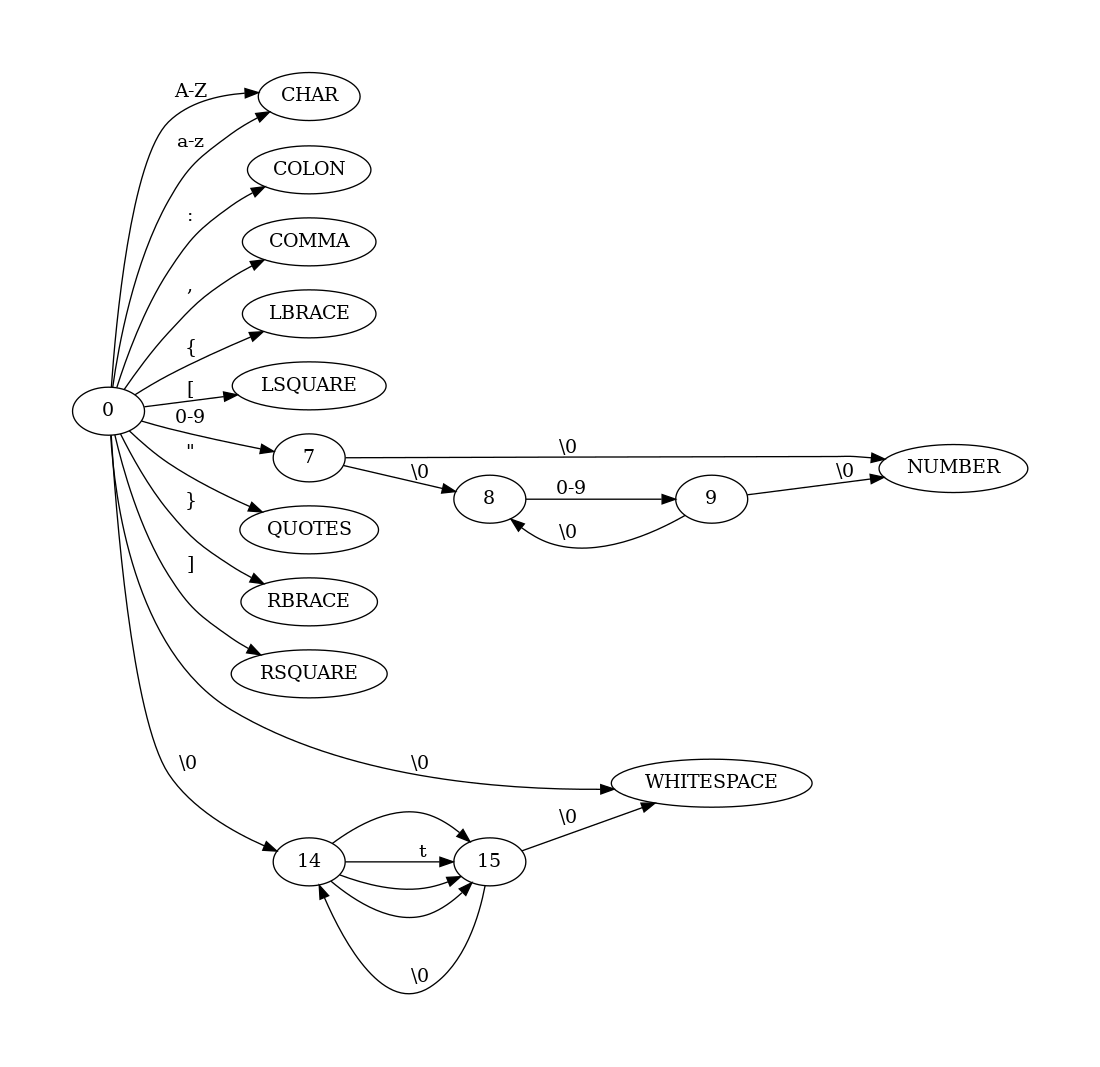
\includegraphics[width=0.8\textwidth]{images/nfa.png}
\caption{NFA of the JSON lexical grammar. The empty string, which is typically denoted with $\epsilon$, is denoted here with \textbackslash0.}
\label{fig:nfa}
\end{figure}

\begin{figure}[t]
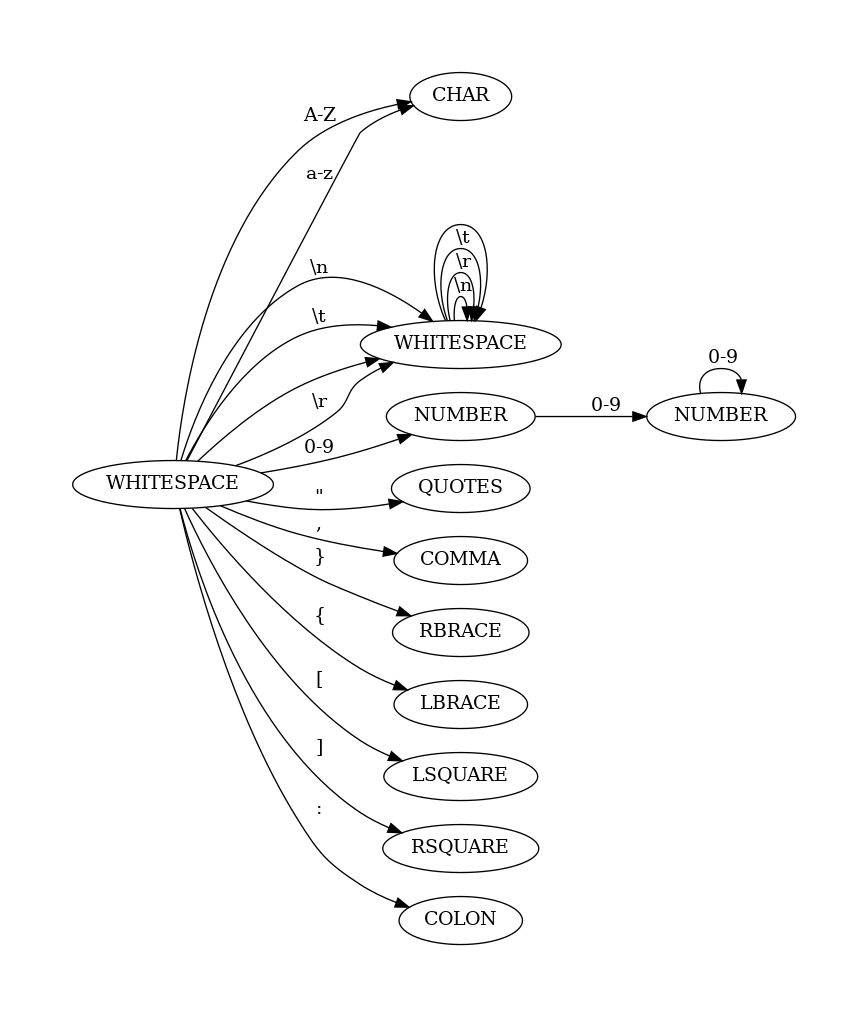
\includegraphics[width=0.8\textwidth]{images/dfa.png}
\caption{DFA of the JSON lexical grammar}
\label{fig:dfa}
\end{figure}

Lexical analysis is performed by processing each character of the input and feeding it into each
lexer instance. Since only the analyzers that begin at a potentially correct start state will
process the input without error, if a lexer instance does encounter an error, it no longer needs
to be processed. 

Each analyzer works by the taking its current state and input symbol and using it to get a new state
from the state transition table. If there is no state for the given state-symbol pair, the instance
checks whether its current state is a terminal state and emits the corresponding lexeme. If there is
not state it can transition to and there is no lexeme to emit, the lexer reaches an error state and
no longer accepts input. 

Once the input has been processed, the outputs from each group lexer instances is placed in the
output skiplist. Once the whole work queue is empty and threads have terminated, the array of
outputs is joined together into one array of lexemes. This is done by iterating over the list and
choosing the outputs that completed analyzing successfully and have the same inital state as the
previous outputs final state. This array of lexemes is then passed onto the syntactic analyzer.

\subsection{Syntactic Analysis}

Syntactic analysis is performed by following the algorithm described in
\cite{barenghi_parallel_2015}. It is a standard  operator precedence parsing algorithm that is
modified to allow for non terminals. Similarly to the lexer, this algorithm requires two passes over
the input. The first pass splits the source string into chunks. Each chunk is assigned to a separate
worker and when all chunks are parsed then the outputs are recombined. Each output consists of a
parse tree, possibly with leading and trailing lexemes that couldn't not be reduced by the parser.
Each two consecutive outputs are then merged such that parsing can continue on the merged whole.
This continues until the parse tree is complete.

\begin{figure}[h]
	\begin{subfigure}[t!]{0.5\textwidth}
	    \centering
	    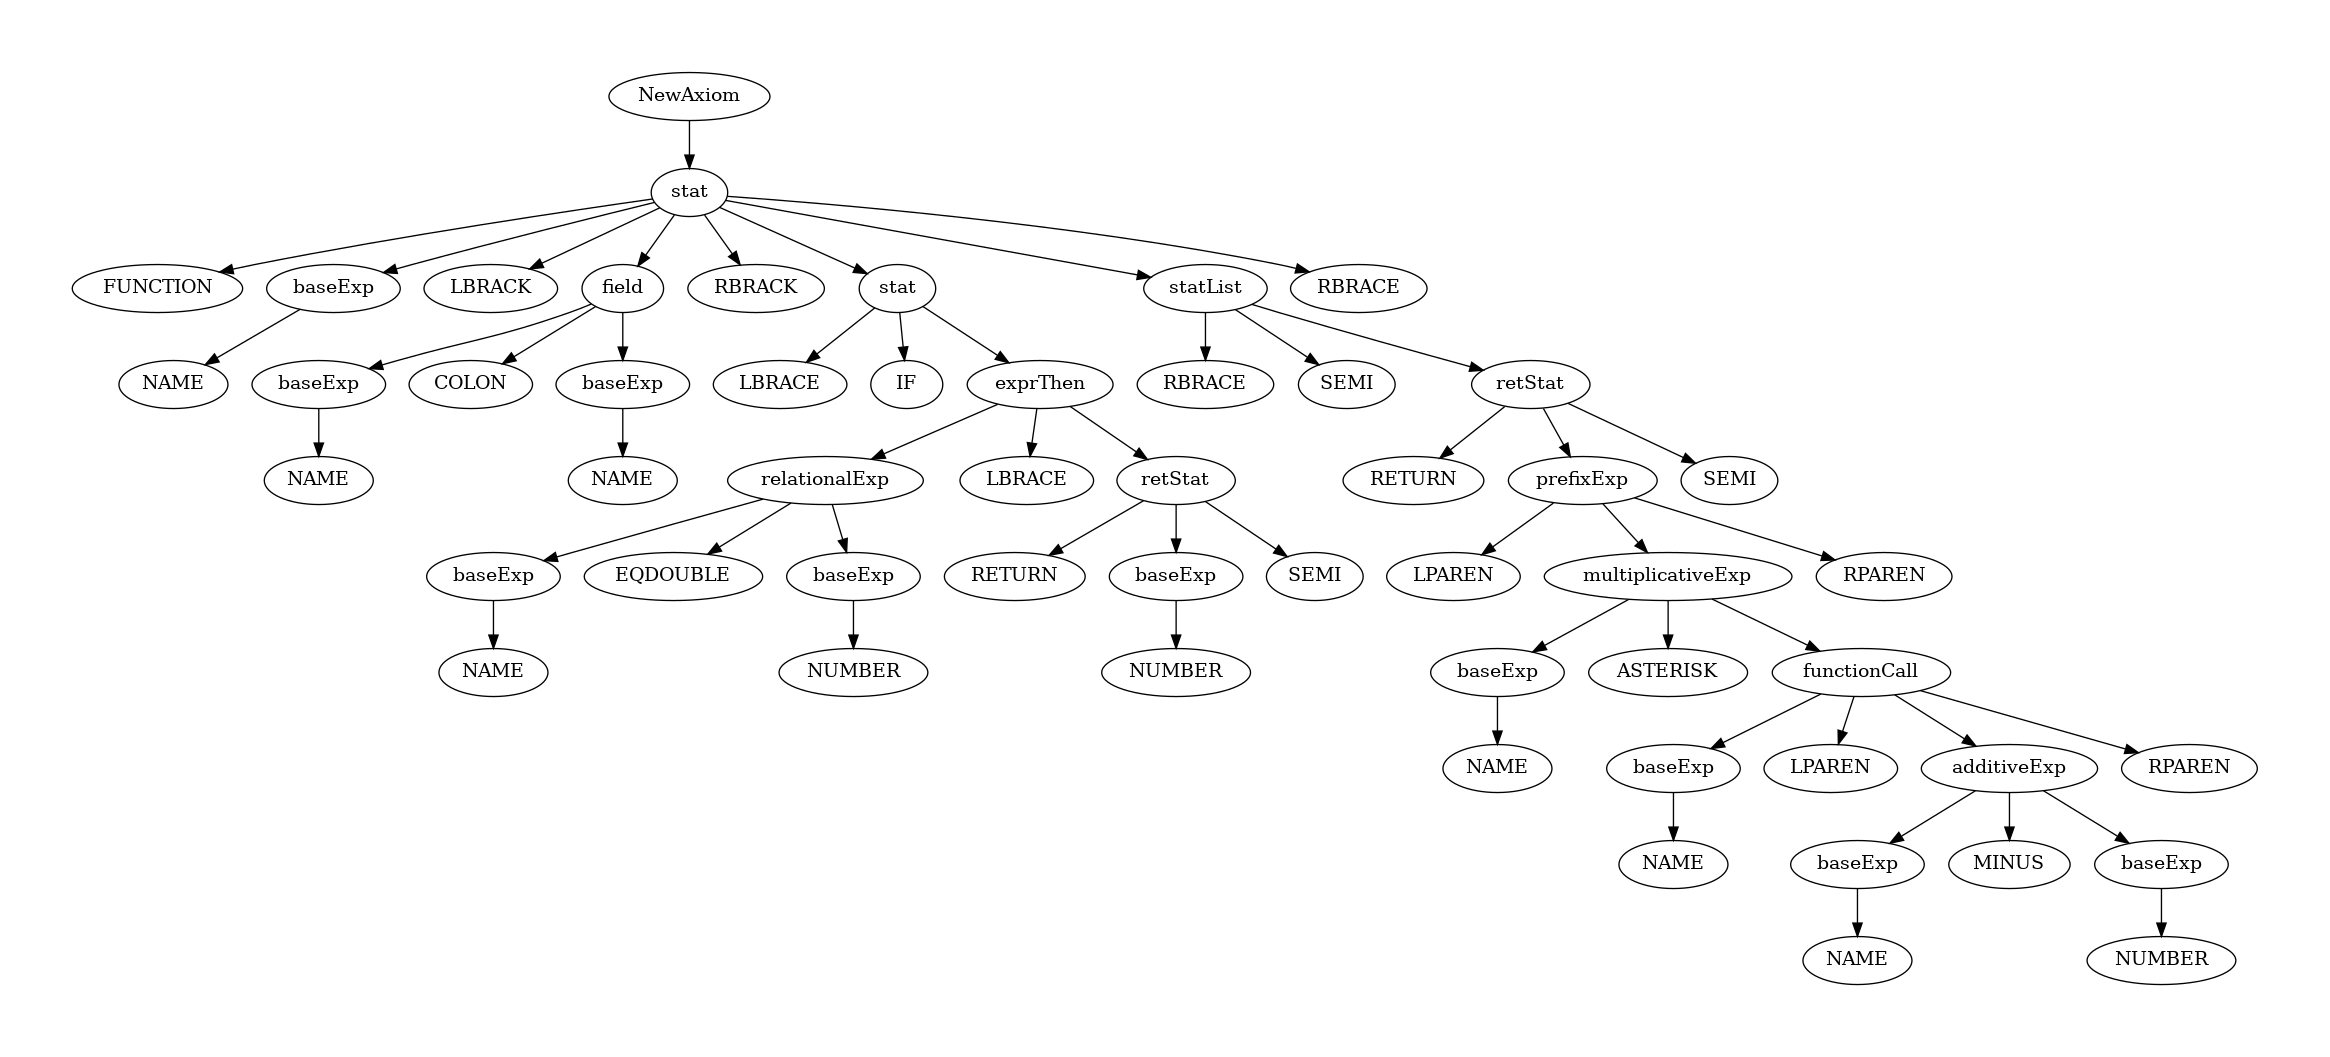
\includegraphics[width=\textwidth]{images/ptree.png}
	\end{subfigure}
	\begin{subfigure}[t!]{0.5\textwidth}
	\centering
	\begin{minted}[breaklines=true, fontsize=\scriptsize]{text}
fn add[a: int, b: int] {
	return a + b;
}
	\end{minted}
	\end{subfigure}%
	\caption{Visualization of the parse tree on the left with the source code on the right. Terminals are capitalised and nonterminals are in camel case.}
	\label{fig:parse_tree}
\end{figure}

\section{Test Langauge Processing} \label{test_lang}

The implementation described thus far can analyse a simple language, such as \gls{json}, without any
modification. All that needs to be specified is a lexing and parsing grammar. This it not the case
with the test langauge due to limitations in the lexing and parsing algorithms.

The syntax of a typical programming language consists of a nested list of statements. Since the
parser requires a terminal between every two non-terminals, any list of of such statements requires
some kind of non-terminal delimeter. A natural choice for this for delimiter is the semicolon
becasue it is also used for this purpose in other programming langauges. An issues arises however
when one considers if, while and function definition statements. Each of these statements unexpectedly requires a semicolon its end. This is very cumbersome and requires that the lexer insert semicolons between pairs , such as between right curly brackets and any lexeme that a statement can begin with.

Another issue I encountered is ditinguising between a unary and binary minus. The parser on
its own is incapable of disovering this distinction because it can potentially lack the context
surrounding a minus lexeme. For example, if the expression $a - b$ were to be parsed starting from
the $-$ symbol, the parser would incorrectly assume that $-$ is a unary operator with $b$ as the
operand. My solution is to emit a different lexeme during lexical analyzer depending on whether any
whitespace was encountered between the a minus sign and the subsequent lexeme.

Due to a limitation of the regular expression parser that is used to read the lexical grammar,
it is not possible to use the look-back regular expression operator. This makes it impossible to
recognise whether an input string is an identifier or a key word of the language in the current
implemetnation. I work around this by defining the keywords separately from the main lexical grammar
and creating a second transtition table from them that is then used to re-analyze any lexemes that
could be a key word of the language.

Semantic analysis of the \gls{ast} checks whether all variables have been used and defined according
to standard scoping rules.

\section{Online Compiler} \label{test_lang}

I decided to create an online compiler demonstration in order to visualize the compiler's outputs
with a graphical user interface. This was made possible by the Rust compiler's ability to compile
code into web assembly. The online compiler executes entirely client side without the need to run
code on a remote server. Webassembly lacks multi-threading capabilities and as such
the demonstration is entirely single threaded.

\section{Dependencies} \label{dependancies}

Code dependencies in the Rust code ecosystem that are  available through the cargo package manager
are called crates. These crates are comparable to small, open source, third party libraries that can
easily be integrated into a rust project. In this section I mention the code dependencies I've used
in my implementation in order to illustrate what parts of my project were accomplished through the
use of third party code.

\subsection{Core}

\textbf{crossbeam} - Common data structures for implementing parallel systems.
This crate implements a concurrently accessible queue, skiplist and a
multi-producer, multi-consumer message passing channel. All of these data
structures are important for reliably sharing data across threads.
\newline\newline
\textbf{regex-syntax} - A crate for parsing standard regular expression syntax.
It provides a simple \gls{ast} that the lexer uses to read the mappings from
lexemes to regular expression patterns.
\newline\newline
\textbf{dot} - A crate that makes it easier to generate graphs in the dot
language. Its used to visualise the parse tree and \gls{ast}.
\gls{ast}.
\newline\newline
\textbf{criterion} - Reliable benchmarking facilities for testing the performance of the
compiler with differently sized inputs.

\subsection{Utility or Minor Contribution}
\textbf{tinyrand} - A lightweight implementation of random number
generation. It is used for creating unique IDs for bathes of work in the work
queue.
\textbf{serde} - Serialization and deserialization capabilities for transferring
code to and from the javascript runtime when running in the browser.
\newline\newline
\textbf{wasm-bindgen} - Macro's for easily creating bindings to javascript when
compiling to web assembly.
\newline\newline
\textbf{log, flexi\_logger ,wasm\-logger, console\_error\_panic\_hook} - Various
crates for logging to files as well as to the terminal, improved formatting and
correct logging when running in the browser.
\newline\newline
\textbf{simple-error} - A simple library for creating errors from error messages
instead of creating types for every error.

\subsection{Optimisation}
\textbf{memmap} - An interface for using linux's memmap syscall. Using memap to
read large files is  faster than using the standard read syscall.
\newline\newline
\textbf{bittyset} - A set implementation that uses a bit vector as a backing
store. This enables a compact representation as well as faster set operations in
the parser where sets of terminals and non-terminals are used.



\newpage
\section{Evaluation And Testing} \label{evalandtesting}
\cite{komathukattil_evaluating_nodate}
\subsection{Unit Testing}
\subsection{Integration Testing}
\subsection{Benchmarks}
\subsection{Alternative}


\newpage
\chapter{Conclusion} \label{conclusion}

\newpage
\end{sloppypar}
\clearpage
\bibliography{references}
\end{document}
